\documentclass[a4paper,11pt]{article}

% --- Packages generaux --------------------------------------------------------
\usepackage[utf8]{inputenc}
\usepackage{textcomp}
\usepackage{lscape}
\usepackage{ucs}
\usepackage[T1]{fontenc}
%\usepackage{eurosym}
%\usepackage{fullpage}
\usepackage{graphicx}
\usepackage[english]{babel}
%\graphicspath{{photos/}{schemas/}}
\usepackage[hidelinks]{hyperref}
\usepackage{pdfpages}

% --- Package specifiques ------------------------------------------------------

%\usepackage{amsmath,amssymb} % pour la gestion facile des trucs orientes maths
\usepackage{listingsutf8} % pour introduire du code source
%\lstloadlanguages{Java}
\usepackage{verbatim}
\usepackage{url}
\usepackage{multicol} % pour les environnement a plusieurs colonnes
\usepackage{vmargin} % pour regler finement les marges (ne pas combiner avec fullpage)
\usepackage{fancyhdr} % pour des en-tetes plus pousses

\usepackage{listings}
\usepackage{color}

\definecolor{dkgreen}{rgb}{0,0.6,0}
\definecolor{gray}{rgb}{0.5,0.5,0.5}
\definecolor{mauve}{rgb}{0.58,0,0.82}

% --- Mise en forme ------------------------------------------------------------

\setlength{\parindent}{7mm}
\setmarginsrb{25mm}{20mm}{25mm}{20mm}{14pt}{5mm}{0pt}{7mm}
% marges gauche, haut, droite, bas
% hauteur de l'entête
% distance entre l'entête et le texte
% hauteur du pied de page
% distance entre le texte et le pied de page

\setcounter{secnumdepth}{3}

\pagestyle{fancy}
\fancyhead[L]{Projet GSI - Cahier des charges - 2016}
\fancyhead[R]{\leftmark}

\lstset{
         basicstyle=\footnotesize\ttfamily, % Standardschrift
         numbers=left,               % Ort der Zeilennummern
         numberstyle=\tiny,          % Stil der Zeilennummern
         %stepnumber=2,               % Abstand zwischen den Zeilennummern
         numbersep=5pt,              % Abstand der Nummern zum Text
         tabsize=2,                  % Groesse von Tabs
         extendedchars=true,         %
         breaklines=true,            % Zeilen werden Umgebrochen
         keywordstyle=\color{red},
    		frame=b,         
         %keywordstyle=[1]\textbf{},    % Stil der Keywords
         %keywordstyle=[2]\textbf{},    %
         %keywordstyle=[3]\textbf{},    %
        %keywordstyle=[4]\textbf{},  % \sqrt{\sqrt{}} %
         stringstyle=\color{white}\ttfamily, % Farbe der String
         showspaces=false,           % Leerzeichen anzeigen ?
         showtabs=false,             % Tabs anzeigen ?
         xleftmargin=17pt,
         framexleftmargin=17pt,
         framexrightmargin=5pt,
         framexbottommargin=4pt,
         %backgroundcolor=\color{lightgray},
         showstringspaces=false      % Leerzeichen in Strings anzeigen ?        
 }

% --- Macros generales ---------------------------------------------------------

% macros pour la page de titre
\newcommand*{\HRule}{\rule{\linewidth}{0.4mm}}  % trait horizontal epais
\newcommand*{\auteur}[2]{\large #1~\textsc{#2}} % mise en forme du nom d'auteur

% tableaux
\newcommand*{\alignloc}[2]{\multicolumn{1}{|#1|}{#2}} % change l'alignement

% macros pour gerer les choses a faire lors de l'ecriture du tex
\newcommand*{\tocheck}{\textcolor{red}{\bf \emph{A VERIFIER}}}
\newcommand*{\checked}{\textcolor{green}{\bf \emph{(vérifié)}}}
\newcommand*{\todo}[1]{\textcolor{blue}{[A FAIRE : \emph{#1}]}}

% --- Mots mal coupes ----------------------------------------------------------

\hyphenation{} % separer les syllabes par des tirets

% --- Elements de la page de titre ---------------------------------------------

\newcommand{\pretitre}{École Internationale des Sciences du Traitement de l'Information (EISTI)}
\newcommand{\grostitre}{GSI Project specifications} 
\newcommand{\auteurs}{Auteurs : \auteur{Titouan}{Bion}, \auteur{Axel}{Martin} et \auteur{Thomas}{Viau} \\ Second year engineering students at the EISTI (Pau).}
\newcommand{\correcteurs}{A l'attention de M. \auteur{Juan}{Angel Lorenzo del Castillo}}
\newcommand{\madate}{\today} % \today pour mettre la date a la compilation

% ==============================================================================
\begin{document}
% ==============================================================================

% --- Page de titre personnalisee ----------------------------------------------

\begin{titlepage}
\begin{figure}[h]

\includegraphics[scale=1]{images/Logo_EISTI.jpg}
\hfill
\end{figure}
  \begin{center}
    ~
    \vfill
    {\large\pretitre\\}           % pre-titre
    \vspace{2cm}
    \HRule \\[0.4cm]
    {\Huge\bf\grostitre\\[0.4cm]} % gros titre
    \HRule \\[0.4cm]
    \vspace{2cm}
    \auteurs\\                    % auteur(s)
    \medskip
    \vfill
   	\correcteurs
    \vfill
    {\large\madate}               % date
  \end{center}
\end{titlepage}

% --- Table des matieres -------------------------------------------------------


\tableofcontents

\newpage

\section{Introduction}

As part of our Parallel Programming and Network courses, we are asked to develop a job scheduler. This document is the specifications of this project.\\
A scheduler is used to assign a job --- processes, threads, etc. --- to the machine hardware resources such as processors. All Operating Systems works with its own scheduler in order to give the user the impression of fluidity even if tons of process are working \textit{"at the same time"}.\\
First, we will present the features of our program. Then we will elaborate on the Queue management and finally we will develop on our chosen scheduling strategy.

\newpage

\section{Features description}

\subsection{What will be implemented?}

We will implement a \texttt{C++} Job Scheduler.\\
To begin with, let's clarify the definition of a job.
A job will be a program launch by a command line. The latter will be given to our application --- along with some parameters\footnote{See \ref{job_parameters} for more information on job parameters.} --- by being added to the Job Queue.

\subsubsection{Job Queue management}

A path to a file that contains all jobs information will be provide to our scheduler at start-up. All jobs included in this file will be processed by our scheduler.\\ However, we will provide a tool to interact with the scheduler to add new job on the fly\footnote{See our Job Queue implementation details for more information: \ref{jobctl_implementation}}.
Jobs will be feed into the Job Queue regardless of the way it have been added and be processed by our program.

\subsubsection{Multiple versions}

First, we will develop a sequential management of our Job Queue, each job will be processed one by one and assigned to available resources according to their priorities\footnote{See our Scheduling Method for more information: \ref{scheduling_strategy}}.\\
Then, we will provided a parallel version of our program to improve our Queue management and processing onto multiple cores of our processor with "OpenMP" library.\\
Finally, we will distribute the last version to a cluster of machine in order to make our program scalable with "MPI" library.

\subsection{Gantt chart}

\todo{compléter diagramme de Fantt}
\todo{Intégrer Gantt}


\newpage

\section{Job Queue implementation details}\label{job_queue_implementation_details}

\subsection{Job parameters}\label{job_parameters}

A job will eventually have different properties --- this list is not exhaustive and may differ at the end --- provided by the user:

\begin{itemize}
\item Burst time [required]
\item Priority
\item RAM and CPU load
\end{itemize}

\todo{explainations}

\subsection{Job Queue parameters}

Despite the fact that our program could work perfectly with default values and use the best for the system, the Job Queue itself can have optional properties. These properties will be provided by the user:
\begin{itemize}
\item \texttt{Timeout}: the time after which the application will kill the job, by default there is no timeout and no job will be killed
\item \texttt{Number of cores}: the number of processors the scheduler can send jobs to, by default it uses different values, depending on the version of the scheduler. In the sequential version it could not be modified and will be set to 1. In the parallel and distributed version it will match the number of available processors.
\item \texttt{Time Slice}: if set to \texttt{0}, there will be no time slice and the scheduler will be non-preemptive\footnote{See our Scheduling Method for more information: \ref{scheduling_strategy}}.
\end{itemize}

\subsection{Dynamic feed of the Job Queue using \texttt{jobctl}}\label{jobctl_implementation}

A tool, \texttt{jobctl}, will be developed in order to interact with the scheduler. This tool will take as parameters the same information required to launch a job. It will then send a \texttt{SIGUSR1} signal to the scheduler, announcing the latter that it needs to reload its job queue. You can see an illustrated version of this routine on Figure \ref{jobctl_implementation_png}. \texttt{jobctl} will also allow the user to see the current state of the processors --- i.e. which job run on this processor.\\
The first implementation will use a swap file in order to add the jobs to the scheduler in real time. The swap file used for the job description and the communication between the client and the scheduler should not be edited by the user.\\
We may lately design a complete API in the scheduler daemon for retrieving or sending other informations such as the cores numbers in the cluster, parametrize the cluster or even remove process.

\begin{center}
\begin{figure}[h]
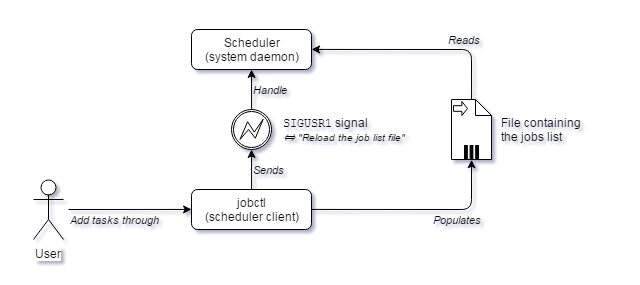
\includegraphics[width=1\linewidth]{images/use_case.png}
\caption{Chart of our Queue implementation.}
\label{jobctl_implementation_png}
\end{figure}
\end{center}


\section{Scheduling strategy}\label{scheduling_strategy}

\subsection{Scheduling method description}

\todo{read and mistakes !}

There are many methods and as many algorithms to achieve scheduling. We chose the fastest method but the most complex to imagine, this is the method used by the majority of Operating Systems, as Windows and UNIX systems (Mac, Linux ..).

This method named Fixed-priority pre-emptive scheduling will always execute the job with the highest priority to ensure that the user can have what he wants first. A job not being prioritized by the user will have a 'default' priority. 
In the case where there are no jobs prioritized and several 'default' priority jobs, the first job that will be executed is the one with the shortest 'burst time' --- the time the job will use for the CPU to compute the job --- to ensure the velocity of the method. 
We will also implement the concept of 'aging' priority too. A process will not wait forever in an infinite loop as the time elapsed since job's declaration will raise the job's priority. For instance, a job with 'default' priority, a burst time of 600ms which was declared for 10s, will be run \textbf{before} a job with 'default' priority, a burst time of 550ms which was declared for 4s.


Moreover, the concept of 'time slice' is used in this method too. It means that a job will not hog the processor for a time longer than the 'time slice'. When a job is being runned by the scheduler, it can be suspended if a job with higher priority comes in, it will be resumed after the termination of the job with higher priority. Indeed, this 'priority race' is checked each 'time slice'. It can be turned off to become a Fixed-priority non-preemptive scheduling, but the pre-emptive method is the one we will use to ensure different jobs can be executed “simultaneously”.


There will be 3 different versions of the application's scheduler, the 3 of them will be available through options.
The 'Sequential', the most basic one, which only allow scheduling on 1 processor
The 'OpenMP', the multi-processors one, which allow using more than 1 processor to start jobs simultaneously
The 'MPI', the scheduler based on clusters, with many processors available on different machines


\subsection{Example of scheduling with our strategy}

The following chart (Figure \ref{scheduling_example}) shows how processes are assigned to cores of a processor. Here we have a duo-core processor with four processes:

\begin{itemize}
\item A $\rightarrow$ Burst time: 300ms ; declared for 3s ; priority: high
\item B $\rightarrow$ Burst time: 100ms ; declared for 2s ; priority: high
\item C $\rightarrow$ Burst time: 200ms ; declared for 2s ; priority: normal
\item D $\rightarrow$ Burst time: 100ms ; declared for 2s ; priority: normal
\end{itemize}

\begin{center}
\begin{figure}[h]
\includegraphics[width=1\linewidth]{images/scheduler_example.png}
\caption{Example of scheduling following our strategy.}
\label{scheduling_example}
\end{figure}
\end{center}

%C'est bon, mais fais gaffe parce que C c'est limite, normalement D devrait passer avant, si le Burst Time est plus petit, on prend celui-là, même si l'autre est en WAITING, donc logiquement on devrait prendre D, sauf que là il est là depuis plus longtemps, donc avec le aging, sa priorité monte un peu + une partie de son burst time a viré, donc C passe avant D mais c'est limite
\newpage

\section{Conclusion}

\todo{formuler}

\newpage

% ==============================================================================
\end{document}
% ==============================================================================
